%!Tex Root = ../Tutorat5.tex
% ./Packete.tex
% ./Design.tex
% ./Deklarationen.tex
% ./Aufgabe2.tex
% ./Aufgabe3.tex
% ./Bonus.tex

% \section{Task 1}
%
% \setcounter{task}{1}
% \begin{frame}{Task 1}{Dynamic Voltage Scaling and Dynamic Power Management}
%     \begin{tasknoinc}
%         What does the constant term in the power consumption $P(f)$ represent? Where does this term come from?
%     \end{tasknoinc}
% \end{frame}
% \begin{frame}{Task 1}{Dynamic Voltage Scaling and Dynamic Power Management}
%     \begin{solutionnoinc}
%         \begin{figure}
%             \centering
%             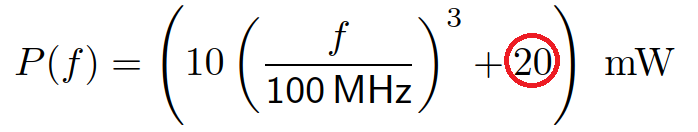
\includegraphics[scale=0.3]{figures/constantTerm.PNG}
%         \end{figure}
%     \begin{itemize}
%         \item The constant term in power consumption represents the minimal power the processor consumes while on.
%         \item That is, power that is drawn even though no gates are being switched (the processor is idling).
%         \item As seen in the lecture, a non-negligible threshold voltage $V_t$ and junction leakage are significant contributors to the minimal power. Gate-oxide leakage also contributes to the static power but it is a lot smaller than the other two components.
%     \end{itemize}
%     \end{solutionnoinc}
% \end{frame}
% \begin{frame}{Task 1}{Dynamic Voltage Scaling and Dynamic Power Management}
%     \begin{solution}
%     \begin{figure}
%         \centering
%         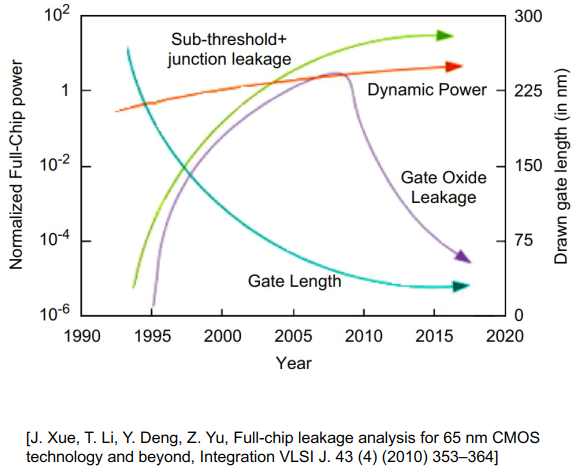
\includegraphics[scale=0.4]{figures/gateLeakages.PNG}
%     \end{figure}
%     \end{solution}
% \end{frame}
% \begin{frame}{Task 1}{Dynamic Voltage Scaling and Dynamic Power Management}
%     \begin{tasknoinc}
%     The energy consumption to execute $C$ cycles is $\frac{C}{f} \cdot P(f)$. There is a critical frequency $f_{crit}$ between 50 MHz and 1000 MHz at which the energy consumption per cycle $\frac{P(f)}{f}$ is minimized. What is the critical frequency $f_{crit}$ of this processor?
%     \end{tasknoinc}
% \end{frame}
% \begin{frame}{Task 1}{Dynamic Voltage Scaling and Dynamic Power Management}
%     \begin{solutionnoinc}
%         \begin{itemize}
%             \item We want to minimize the energy consumption per cycle $(\frac{P(f)}{f})$ with respect to the frequency $f$. By doing this, we will find $f_{crit}$.
%             \item First, we define $f_n := \frac{f}{100 MHz}$ to be the normalized frequency. We are doing this for easier calculation.
%             \item We then define the energy consumption per cycle as $Q(f_n) := \frac{P(f_n)}{f_n} = \frac{10f_n^3+20}{f_n} = 10f_n^2 + \frac{20}{f_n}$
%             \item The first term \alert{decreases}, the second term \alert{increases} when reducing $f_n$!
%             \item The latter is a result of the increasing execution time of a cycle when decreasing the frequency, the processor has to be on for a longer time.
%         \end{itemize}
%     \end{solutionnoinc}
% \end{frame}
% \begin{frame}{Task 1}{Dynamic Voltage Scaling and Dynamic Power Management}
%     \begin{solution}
%         \begin{itemize}
%             \item Calculating the derivative of $Q(f_n)$ we obtain $20f_n - \frac{20}{f_n^2}$
%             \item This equals 0 for $f_n = 1$, meaning $\frac{f_{crit}}{100 MHz} = 1$. Therefore we know, that the critical frequency is $f_{crit} = 100 MHz$.
%         \end{itemize}
%     \end{solution}
% \end{frame}
% \begin{frame}{Task 1}{Dynamic Voltage Scaling and Dynamic Power Management}
%     \begin{tasknoinc}
%         When the processor is idle at frequency $f_{min}$ for $t$ seconds, the consumed energy is $P(f_{min}) \cdot t$. The break-even time is defined as the minimum idle interval, for which it is worthwhile for the processor to go into sleep mode. What is the break-even time of the processor?
%     \end{tasknoinc}
% \end{frame}
% \begin{frame}{Task 1}{Dynamic Voltage Scaling and Dynamic Power Management}
%     \begin{solutionnoinc}
%         \begin{itemize}
%             \item To break even we need to consider both the costs for staying in a certain mode and the costs of switching between modes.
%             \item The point we search means, that the consumed energy for switchting to sleep, staying in sleep and switching back to run needs to be at most $P(f_{min}) \cdot t$.
%             \item Since we do not consider switching times, and we assume that modes can be switched without any time passing, we can neglect that time factor.
%             \item In total, this means we get the following inequality: $P(f_{min}) \cdot t \geq E_{RunToSleep} + E_{sleep} + E_{SleepToRun}$
%         \end{itemize}
%     \end{solutionnoinc}
% \end{frame}
% \begin{frame}{Task 1}{Dynamic Voltage Scaling and Dynamic Power Management}
%     \begin{solutionnoinc}
%         \begin{itemize}
%             \item $P(f_{min}) \cdot t \geq E_{RunToSleep} + E_{sleep} + E_{SleepToRun}$
%             \item We know that the energy consumption from switching to run to sleep is 0, same for the energy consumption when idling in sleep. The energy consumption for switching from sleep to run is $30 \mu J$.
%             \item Thus, the above inequality is\\ $P(f_{min}) \cdot t \geq 30 \mu J$
%             \item[]
%             \item[] $t \geq \frac{30 \mu J}{(10 * 0.5^3 + 20)mW}$
%             \item[]
%             \item[] $t \geq 1.412ms$
%         \end{itemize}
%     \end{solutionnoinc}
% \end{frame}
% \begin{frame}{Task 1}{Dynamic Voltage Scaling and Dynamic Power Management}
%     \begin{solution}
%         \begin{itemize}
%             \item The break-even time is the minimal time for which the inequality holds and therefore $t_{break\text{-}even} = 1.412 ms.$
%         \end{itemize}
%     \end{solution}
% \end{frame}
% \begin{frame}{Task 1}{Dynamic Voltage Scaling and Dynamic Power Management}
%     \begin{tasknoinc}
%     A workload-conserving schedule is defined as a schedule that is always executing a job when the ready queue is not empty. For the three jobs above, provide the workload-conserving schedule that minimizes the energy consumption without violating the timing constraints. For this subquestion, all tasks are executed at critical frequency $f_crit = 100 MHz$. What is the energy consumption of this schedule?
%     \end{tasknoinc}
% \end{frame}
% \begin{frame}{Task 1}{Dynamic Voltage Scaling and Dynamic Power Management}
%     \begin{solutionnoinc}
%         \begin{figure}
%             \centering
%             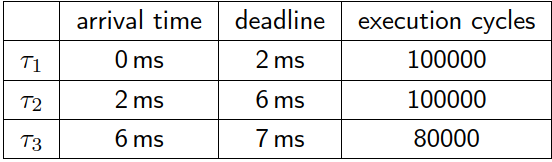
\includegraphics[scale=0.5]{figures/jobsToExecute.PNG}
%         \end{figure}
%         \begin{itemize}
%             \item For this question it is important to check if the processor should switch to sleep mode between tasks or not. Frequency switching has negligible overhead, meaning when not executing a task we can let the processor idle with frequency $f_{min}$.
%             \item This means we can use the break-even point as calculated in task (c).
%             \item The execution times for $\tau_1, \tau_2$ and $\tau_3$ are $1ms, 1ms$ and $0.8ms$ respectively.
%         \end{itemize}
%     \end{solutionnoinc}
% \end{frame}
% \begin{frame}{Task 1}{Dynamic Voltage Scaling and Dynamic Power Management}
%     \begin{solutionnoinc}
%         \begin{figure}
%             \centering
%             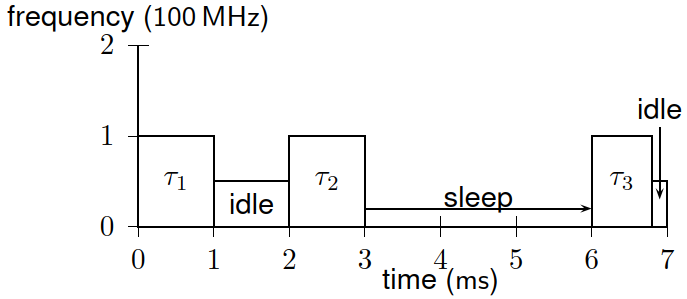
\includegraphics[scale=0.5]{figures/scheduleD).PNG}
%         \end{figure}
%         \begin{itemize}
%             \item The energy consumption of the schedule is $E = \frac{C_{\tau_1}}{f_{crit}} + t_{idle,1} \cdot P(f_{min}) + \frac{C_{\tau_2}}{f_{crit}} \cdot P(f_{crit}) + E_{sleep} + E_{modechange} + \frac{C_{\tau_3}}{f_{crit}} \cdot P(f_{crit})$
%         \end{itemize}
%     \end{solutionnoinc}
% \end{frame}
% \begin{frame}{Task 1}{Dynamic Voltage Scaling and Dynamic Power Management}
%     \begin{solution}
%         \begin{itemize}
%             \item Plugging in the values yields: $E = 0.001s \cdot 30mW + 0.001s \cdot 21.25mW + 0.001s \cdot 30mW + 0J + 30µJ + 0.0008s \cdot 30mW + 0.0002s \cdot 21.25mW = 0.1395 mJ$
%         \end{itemize}
%     \end{solution}
%     \begin{Sidenote}
%     Note that in the time interval [1, 2] we do not go into sleep mode as the interval is smaller than the break-even time. During the idle time intervals [1, 2] and [6.8, 7], we select the minimum frequency $f_{min}$. Since no task is executed then, this choice minimizes power consumption.
%     \end{Sidenote}
% \end{frame}
% \begin{frame}{Task 1}{Dynamic Voltage Scaling and Dynamic Power Management}
%     \begin{tasknoinc}
%     Is there another workload-conserving schedule without timing constraints violations for the three jobs
% that has a lower energy consumption than the schedule in (d)? There are no restrictions at what
% frequency tasks have to be executed. If so, provide the schedule, otherwise prove the optimality of the
% schedule in (d).
%     \end{tasknoinc}
% \end{frame}
%
% \begin{frame}{Task 1}{Dynamic Voltage Scaling and Dynamic Power Management}
%     \begin{solutionnoinc}
%         \begin{itemize}
%             \item Yes! The idea is to use the convex nature of the power consumption to slow down execution of tasks $\au_1$ and $\tau_3$ to avoid idle times after their executions.
%             \item Even though we execute tasks below the critical frequency, the overall consumption is lower.
%             \item We calculate the frequencies for $\tau_1$ and $\tau_3$ to close the idle gaps. Thus, the new frequencies are $f_{\tau_1} = \frac{C_{\tau_1}}{t_{\tau_1}}$ and $f_{\tau_3} = \frac{C_{\tau_3}}{t_{\tau_3}}$ where $t_{\tau_1} = 2ms$ and $t_{\tau_3} = 1ms$.
%         \end{itemize}
%     \end{solutionnoinc}
% \end{frame}
%
% \begin{frame}{Task 1}{Dynamic Voltage Scaling and Dynamic Power Management}
%     \begin{solutionnoinc}
%         \begin{figure}
%             \centering
%             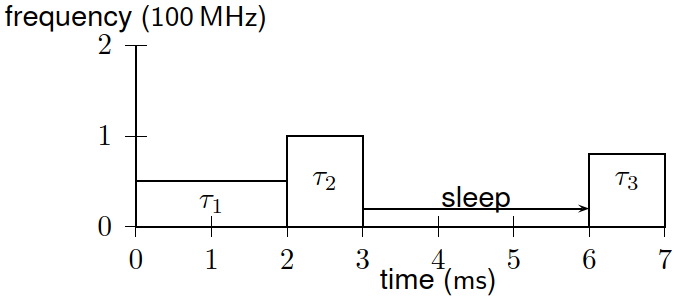
\includegraphics[scale = 0.5]{figures/scheduleE).PNG}
%         \end{figure}
%         \begin{itemize}
%             \item The energy consumption of the schedule is $E = t_{\tau_1} \cdot P(f_{\tau_1}) + \frac{C_{\tau_2}}{f_{crit}} \cdot P(f_{crit}) + E_{sleep} + E_{modechange} + t_{\tau_3} \cdot P(f_{\tau_3})$
%         \end{itemize}
%     \end{solutionnoinc}
% \end{frame}
% \begin{frame}{Task 1}{Dynamic Voltage Scaling and Dynamic Power Management}
%     \begin{solution}
%         \begin{itemize}
%             \item Plugging in the values yields: $E = 0.002s \cdot 21.25mW + 0.001s \cdot 30mW + 0J + 30\mu J + 0.001s \cdot 25.12mW = 0.12762 mJ$
%         \end{itemize}
%     \end{solution}
% \end{frame}
% \begin{frame}{Task 1}{Dynamic Voltage Scaling and Dynamic Power Management}
%     \begin{tasknoinc}
%     Does a schedule for the three jobs without timing constraints violations exist that is not workload-conserving but consumes less energy than the optimal workload-conserving schedule? If so, provide the schedule, otherwise prove the optimality of the workload-conserving schedules.
%     \end{tasknoinc}
% \end{frame}
% \begin{frame}{Task 1}{Dynamic Voltage Scaling and Dynamic Power Management}
%     \begin{solutionnoinc}
%         \begin{itemize}
%             \item Yes! The idea is to batch the inactive time into one block that the processor will spend in sleep mode and execute $\tau_1$ with critical frequency.
%             \item This shows: Workload-conserving strategies are \alert{not} necessarily the best!
%             \item By using this strategie, the processor sleeps a very long time, as we are allowed to delay $\tau_2$, saving energy.
%         \end{itemize}
%     \end{solutionnoinc}
% \end{frame}
% \begin{frame}{Task 1}{Dynamic Voltage Scaling and Dynamic Power Management}
%     \begin{solutionnoinc}
%         \begin{figure}
%             \centering
%             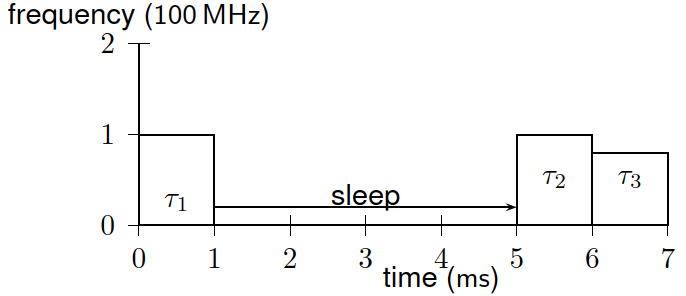
\includegraphics[scale = 0.5]{figures/scheduleF).PNG}
%         \end{figure}
%         \begin{itemize}
%             \item The energy consumption of the schedule is $E = \frac{C_{\tau_1}}{f_{crit}} \cdot P(f_{crit}) + E_{sleep} + E_{mode\ change} + \frac{C_{\tau_2}}{f_{crit}} \cdot P(f_{crit}) + t_{\tau_3} \cdot P(f_{\tau_3})$
%         \end{itemize}
%     \end{solutionnoinc}
% \end{frame}
% \begin{frame}{Task 1}{Dynamic Voltage Scaling and Dynamic Power Management}
%     \begin{solution}
%         \begin{itemize}
%             \item Plugging in the values yields: $E = 0.001s\  \cdot 30mW\  +\  0J\  +\  30\mu J\  +\  0.001s\  \cdot\  30mW\  +\  0.001s\  \cdot\  25.12mW = 0.115120 mJ$
%         \end{itemize}
%     \end{solution}
% \end{frame}

